\bookchapter{Capítulo 37: A revolução de paradigma — de “escrever código” a “comandar a IA a escrever”}

\chapterintro{Parabéns: ao abrir este livro, você está bem no centro de uma revolução de paradigma profissional. O ponto de partida foi uma frase de um programador nas redes sociais, em 2025. Parece dramático? Mas é assim mesmo.}

\booksection{O nascimento do Vibe Coding: um movimento de uma frase}

Em fevereiro de 2025, Andrej Karpathy — guarde este nome, ele ainda aparece várias vezes — publicou um tweet que viraria referência: “Existe um jeito novo de programar chamado Vibe Coding: você vai só no feeling, ignora os detalhes do código e deixa a IA fazer tudo. Diz o que vê, copia e cola; se funcionar, tá ótimo.”

A frase, aparentemente de improviso, batizou com precisão uma mudança de paradigma que já estava acontecendo: em vez de escrever código linha a linha, os humanos descrevem a intenção em linguagem natural e a IA implementa. O tom era brincalhão, mas a percepção era profunda: quando a geração de código pela IA cruza um certo limiar, o gargalo deixa de ser “consigo escrever esta linha?” e passa a ser “sei pensar com clareza sobre o que quero?”.

\begin{tcbinfo}{Dica: o que é "vibe"?}
Vibe é “clima, sensação”. Vibe Coding é “programar guiando a IA pelo feeling” — você descreve o que quer e a IA implementa. Guarde o termo: é a certidão de nascimento da revolução.

\end{tcbinfo}

A partir daí, “codificar” se dividiu em dois sentidos: codificar tradicionalmente é traduzir o design para a sintaxe; codificar novo é traduzir a intenção em instruções. O primeiro testa os dedos; o segundo, a cabeça.

Vibe Coding rapidamente deixou de ser piada e virou conceito de engenharia. Por volta de meados de 2026, já era uma metodologia completa — expressão de requisitos, gestão de contexto, iteração, verificação e qualidade. A gente também percebeu: “programar no feeling” é só a porta de entrada; programação eficiente com IA exige um modo sistemático de pensar. É exatamente isso que este livro vai te dar.

\booksection{O cenário em 2026: a era da Agentic Engineering}

Em agosto de 2026, a programação com IA já tinha passado por várias revoluções de paradigma. O Vibe Coding foi a faísca inicial, mas logo ficou claro: só “conversar no feeling” com a IA gera código instável — às vezes brilhante, às vezes um desastre. O paradigma então evoluiu: da programação conversacional simples para a engenharia estruturada de Agentes.

Karpathy de novo: no início de 2026, ele propôs o conceito de Agentic Engineering. Diferente do “diz e gera” do Vibe Coding, a Agentic Engineering defende: dê um objetivo à IA e deixe que ela planeje os passos, use ferramentas, valide resultados e corrija em ciclo. A IA deixa de ser um gerador de código e vira um agente que percebe o ambiente, decide e age.

Três mudanças-chave:

\begin{enumerate}
  \item Interação: de "pergunta e resposta" para "definir o objetivo e soltar as rédeas".
  \item Entregável: de "um trecho de código" para "um projeto completo".
  \item Papel do humano: de "revisar linha a linha" para "definir limites e validar o resultado".
\end{enumerate}

Os números não mentem: no Cursor 3, lançado em abril de 2026, o modo Agent ultrapassou pela primeira vez o autocomplete por Tab, sinal de que os desenvolvedores migraram em massa. Já o Claude Code, ferramenta de programação com IA nativa de terminal, chegou a US\$ 2,5 bilhões de receita anualizada em meados de 2026. O gráfico abaixo mostra esse momento de virada:

\begin{center}
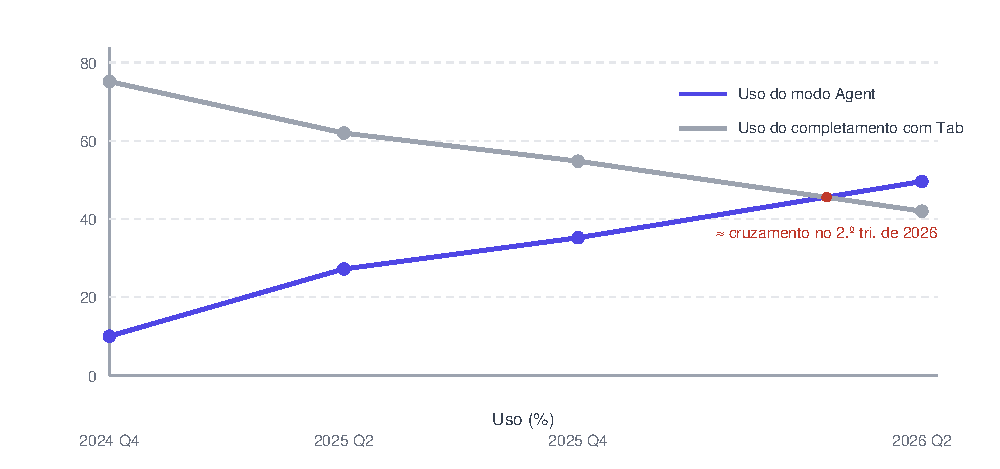
\includegraphics[width=0.92\linewidth]{figures/fig-di-san-shi-qi-zhang-1}
\\[2pt]\small Figura 1: tendência do uso dos modos de interação em programação com IA (estimativa com base em pesquisas do setor; no 2º tri. de 2026, o modo Agent ultrapassa o Tab)
\end{center}

Mas vamos ser francos: ferramentas e modelos são só a superfície. Quer use Cursor ou Claude Code, quer o modelo de base seja GPT-5 ou Claude 4.5, quem tem sucesso com IA segue a mesma metodologia de fundo. É isso que este guia ensina.

\booksection{A virada cognitiva: de Coder a Conductor}

O ensino tradicional de programação forma um Coder: entender sintaxe, decorar API, depurar lógica. Na era da IA, esse papel está sendo redefinido. Você não precisa mais digitar cada linha, mas precisa virar um “maestro” (Conductor): definir o campo de batalha, criar as regras, distribuir tarefas e validar o resultado.

O cerne não é “saber escrever código”, e sim “pensar com clareza o que se quer fazer”. Um bom general não precisa ser o melhor soldado, mas precisa dominar o objetivo da campanha, o terreno e o posicionamento das tropas. Do mesmo modo, quem programa bem com IA não precisa decorar a sintaxe de cada linguagem, mas precisa compreender o objetivo do projeto, as restrições de arquitetura e os padrões de qualidade.

Vale olhar esta tabela duas vezes — ela resume toda a mudança de papel:

\begin{center}
\begin{tabularx}{\linewidth}{|X|X|X|}
\hline
\textbf{Dimensão} & \textbf{Coder tradicional} & \textbf{Conductor de IA} \tabularnewline
\hline
Competências centrais & Sintaxe, chamadas de API, depuração & Definição de requisitos, contexto, critérios de aceite \tabularnewline
Modo de trabalho & Escrever código linha a linha & Descrever a intenção e auditar a entrega \tabularnewline
Controle de qualidade & Se você escreveu, sabe o que há dentro & Validar o que a IA gerou com testes e revisão \tabularnewline
Exigência de conhecimento & Domínio profundo de uma linguagem/framework & Amplitude técnica + profundidade no negócio \tabularnewline
Onde está o gargalo & Velocidade de digitação e memória de sintaxe & Clareza de pensamento e capacidade de expressão \tabularnewline
Origem dos erros & Erros de sintaxe, falhas de lógica & Requisitos vagos, contexto insuficiente \tabularnewline
\hline
\end{tabularx}
\end{center}

\begin{center}\small\color{gray}Comparação entre o Coder tradicional e o Conductor de IA\end{center}

Isso não quer dizer que conhecimento de programação não importa. Pelo contrário: só quem lê o código da IA consegue revisar e corrigir com eficácia; só quem entende estruturas de dados e algoritmos julga se a solução faz sentido. Seu repertório define o “teto de comando” — mas o papel do conhecimento migra de “ferramenta de execução” para “base de julgamento”.

\booksection{Por que a metodologia vale mais que a ferramenta}

Ferramentas mudam a cada três meses; a metodologia evolui a cada três anos. Aprender a operar uma ferramenta pode ficar desatualizado em três meses; dominar um jeito de pensar ainda vale daqui a três anos.

Muita gente que começa em programação com IA já pergunta de cara: “qual é a melhor ferramenta?”, “qual é o modelo mais forte?”. São perguntas válidas, mas na ordem errada. O mercado de agosto de 2026 não tem nada a ver com o de agosto de 2025 — Trae, Qoder e outros sobem e descem; o Cursor virou de plugin a IDE independente e chegou ao Cursor 3; o Claude Code saiu de experimento e virou padrão no terminal. Mas, por trás dessa turbulência, os princípios de quem tem sucesso quase não mudaram.

Por isso este livro não gasta páginas ensinando cliques de uma ferramenta específica — isso envelhece rápido. O foco está em uma metodologia comprovada: como pensar requisitos, como conversar com a IA, como validar entregas, como iterar. Com ela, você se adapta a qualquer ferramenta; sem ela, cada troca recomeça do zero.

\begin{tcbinfo}{Tranquilidade para quem está começando do zero}
Se você é iniciante, não se assuste com a palavra “metodologia”. Não é filosofia abstrata: é um manual de “como pensar quando o problema aparece”. É como cozinhar: dá para seguir a receita passo a passo (operação da ferramenta), mas o bom chef entende “por que este tempero” e “como controlar o fogo” (metodologia). O livro parte do zero e cada princípio vem com casos comparativos, para você entender não só o “o que”, mas o “como”.

\end{tcbinfo}

\begin{tcbpractice}{Mão na massa: tire uma "foto de papel" de quem você é hoje}
Pegue um papel e responda: (1) Como você usa a IA para escrever código hoje (se já usou)? (2) Você se parece mais com o “Coder” ou com o “Conductor” da tabela? (3) Daqui a três meses, como você gostaria de descrever o seu jeito de trabalhar? Guarde o papel no livro e releia depois do Capítulo 47 — a mudança vai ser mais rápida do que você imagina.

\end{tcbpractice}

\begin{tcbsummary}{Resumo do capítulo}
\begin{itemize}
  \item Em 2025, Karpathy batizou a revolução de "Vibe Coding": de código linha a linha para intenção em linguagem natural
  \item Em 2026, evoluímos para a Agentic Engineering: objetivo + autonomia, a IA planeja e executa, o humano valida
  \item No Cursor 3, o modo Agent ultrapassou o Tab; o Claude Code chegou a US\$ 2,5 bi anuais
  \item Seu novo papel é Conductor: definir o campo, as regras, as tarefas e validar os resultados
  \item Ferramentas mudam a cada três meses; metodologia, a cada três anos — aprenda método, não cliques
\end{itemize}

\end{tcbsummary}
